\documentclass[usenames,dvipsnames,t]{beamer}

\usepackage[english]{babel}
\usepackage[utf8]{inputenc}
\usepackage{amsmath,amsthm, amssymb, latexsym}
\usepackage{amssymb}
\usepackage{color}
\usepackage{tikz}
\usepackage{standalone}
\usepackage{minted}
\usepackage{fontawesome}
\usepackage{setspace}
\usepackage{rotating}

\definecolor{DarkGray}{RGB}{5, 66, 81}
\definecolor{DarkerGray}{RGB}{3, 22, 27}

\usemintedstyle{native}

\usetikzlibrary{shapes.arrows, positioning, arrows, decorations.pathreplacing,
angles, quotes, decorations.pathmorphing}
\tikzset{
    ultra thick/.style={line width=3pt}
}
\usetikzlibrary{matrix}

\usecolortheme[dark,accent=cyan]{solarized}
\beamertemplatenavigationsymbolsempty
\setbeamerfont{block title}{size=\Large}
\usepackage[orientation=landscape,size=a1,scale=1.4]{beamerposter}
\newcommand{\R}{\mathbb{R}}

\renewcommand{\arraystretch}{0.8}

\addtobeamertemplate{block begin}{%
  \setlength{\textwidth}{.5\textwidth}%
}{}

\addtobeamertemplate{block alerted begin}{%
  \setlength{\textwidth}{.5\textwidth}%
}{}

\addtobeamertemplate{block example begin}{%
  \setlength{\textwidth}{.5\textwidth}%
}{}
\setbeamerfont{block body}{size=\footnotesize}
%%%%%%%%%%%%%%%%%%%%%%%%%%%%%%%%%%%%%%%%%%%%%%%%%%%%%%%%%%%%%%%%%%%%%%%%%%%%%%%
\begin{document}

%%%%%%%%%%%%%%%%%%%%%%%%%%%%%%%%TITLE%%%%%%%%%%%%%%%%%%%%%%%%%%%%%%%%%%%%%%%%%%%
\begin{columns}
    % \begin{column}{.1\linewidth}
    % \end{column}
    \begin{column}{.7\linewidth}
    \vspace{1.5cm}

    \centering
    \textbf{\textcolor{orange}{\fontsize{110}{120} \selectfont THE POWER OF MEMORY}}
    \vspace{0.7cm}

    \textbf{\Large\textcolor{orange}{Is memory size advantageous in interactions (social,
    biological, $\dots$) ?}}
    \end{column}
    \begin{column}{.2\linewidth}
        
        \begin{center}
            \includestandalone[width=.75\textwidth]{static/matrix}
        \end{center}
        \end{column}
    % \begin{column}{.23\linewidth}

    %     \includestandalone[width=\textwidth]{static/memory_one}
    % \end{column}
    \begin{column}{.02\linewidth}
    \end{column}
\end{columns}
\vspace{1cm}

\hrule height 3pt
\vspace{1cm}

% %%%%%%%%%%%%%%%%%%%%%%%%%%%%%%%%FIRST ROW%%%%%%%%%%%%%%%%%%%%%%%%%%%%%%%%%%%%%%%
\begin{columns}
    \begin{column}{.05\linewidth}
    \end{column}
    \begin{column}{.2\linewidth}
        \vspace{3cm}

        \includestandalone[width=\textwidth]{static/memory_one}
    \end{column}
    \begin{column}{.3\linewidth}
    \vspace{-.5cm}
        \begin{center}
            \includestandalone[width=.45\textwidth]{static/states} \\
            \includestandalone[width=.05\textwidth]{static/arrow_down} \\
            \normalsize{
\(
\left[\begin{matrix}p_{1} q_{1} & p_{1} \left(- q_{1} + 1\right) & q_{1} \left(- p_{1} + 1\right) & \left(- p_{1} + 1\right) \left(- q_{1} + 1\right)\\
p_{2} q_{3} & p_{2} \left(- q_{3} + 1\right) & q_{3} \left(- p_{2} + 1\right) & \left(- p_{2} + 1\right) \left(- q_{3} + 1\right)\\
p_{3} q_{2} & p_{3} \left(- q_{2} + 1\right) & q_{2} \left(- p_{3} + 1\right) & \left(- p_{3} + 1\right) \left(- q_{2} + 1\right)\\
p_{4} q_{4} & p_{4} \left(- q_{4} + 1\right) & q_{4} \left(- p_{4} + 1\right) & \left(- p_{4} + 1\right) \left(- q_{4} + 1\right)\end{matrix}\right]
\)
}
        \end{center}
    \end{column}
    \begin{column}{.1\linewidth}
        \vspace{2cm}

        \includestandalone[width=.7\textwidth]{static/trident_arrow}
    \end{column}
    \begin{column}{.3\linewidth}
        \vspace{1cm}

        \small{
            W. H. Press and F. J. Dyson. \textbf{Iterated Prisoner's
            Dilemma contains strategies that dominate any evolutionary opponent}
            PNAS 2012.%Introducing the zero determinant strategies:
            \[p ^ * \rightarrow \text{ manipulates } \rightarrow q\]
        }
        \vspace{1cm}

        \small{
        This work considers an optimisation approach to identify:
        \[ p ^ * \rightarrow \text{ best response } \rightarrow q\]}
        \normalsize{{
            \boldmath{\[u_q(p)= \frac{\frac{1}{2}\enspace p  Q  p^T + c^T p + a}
                  {\frac{1}{2}\enspace  p  \bar{Q}  p^T + \bar{c}^T  p + \bar{a}},\] \\
                  \[\text{where }  \ p \in \R^4_{[0, 1]}\]
            }}}
    \end{column}
    \begin{column}{.05\linewidth}
    \end{column}
\end{columns}
\vspace{1cm}

\hrule height 3pt
\vspace{1cm}
%%%%%%%%%%%%%%%%%%%%%%%%%%%%%%%%SECOND ROW%%%%%%%%%%%%%%%%%%%%%%%%%%%%%%%%%%%%%%
\begin{columns}
    \begin{column}{.7\linewidth}
        \begin{center}
            \textcolor{orange}{\textbf{\Large{PURELY RANDOM STRATEGIES \(p=(p, p, p, p)\)}}}
        \end{center}

    \begin{columns}
        \begin{column}{.5\linewidth}
            \begin{center}
            \vspace{-1cm}

            \textcolor{orange}{\textbf{\small{AGAINST A SINGLE OPPONENT}}}
            \vspace{2cm}

            \includestandalone[width=.7\textwidth]{static/single_opponent}
            \vspace{2cm}

            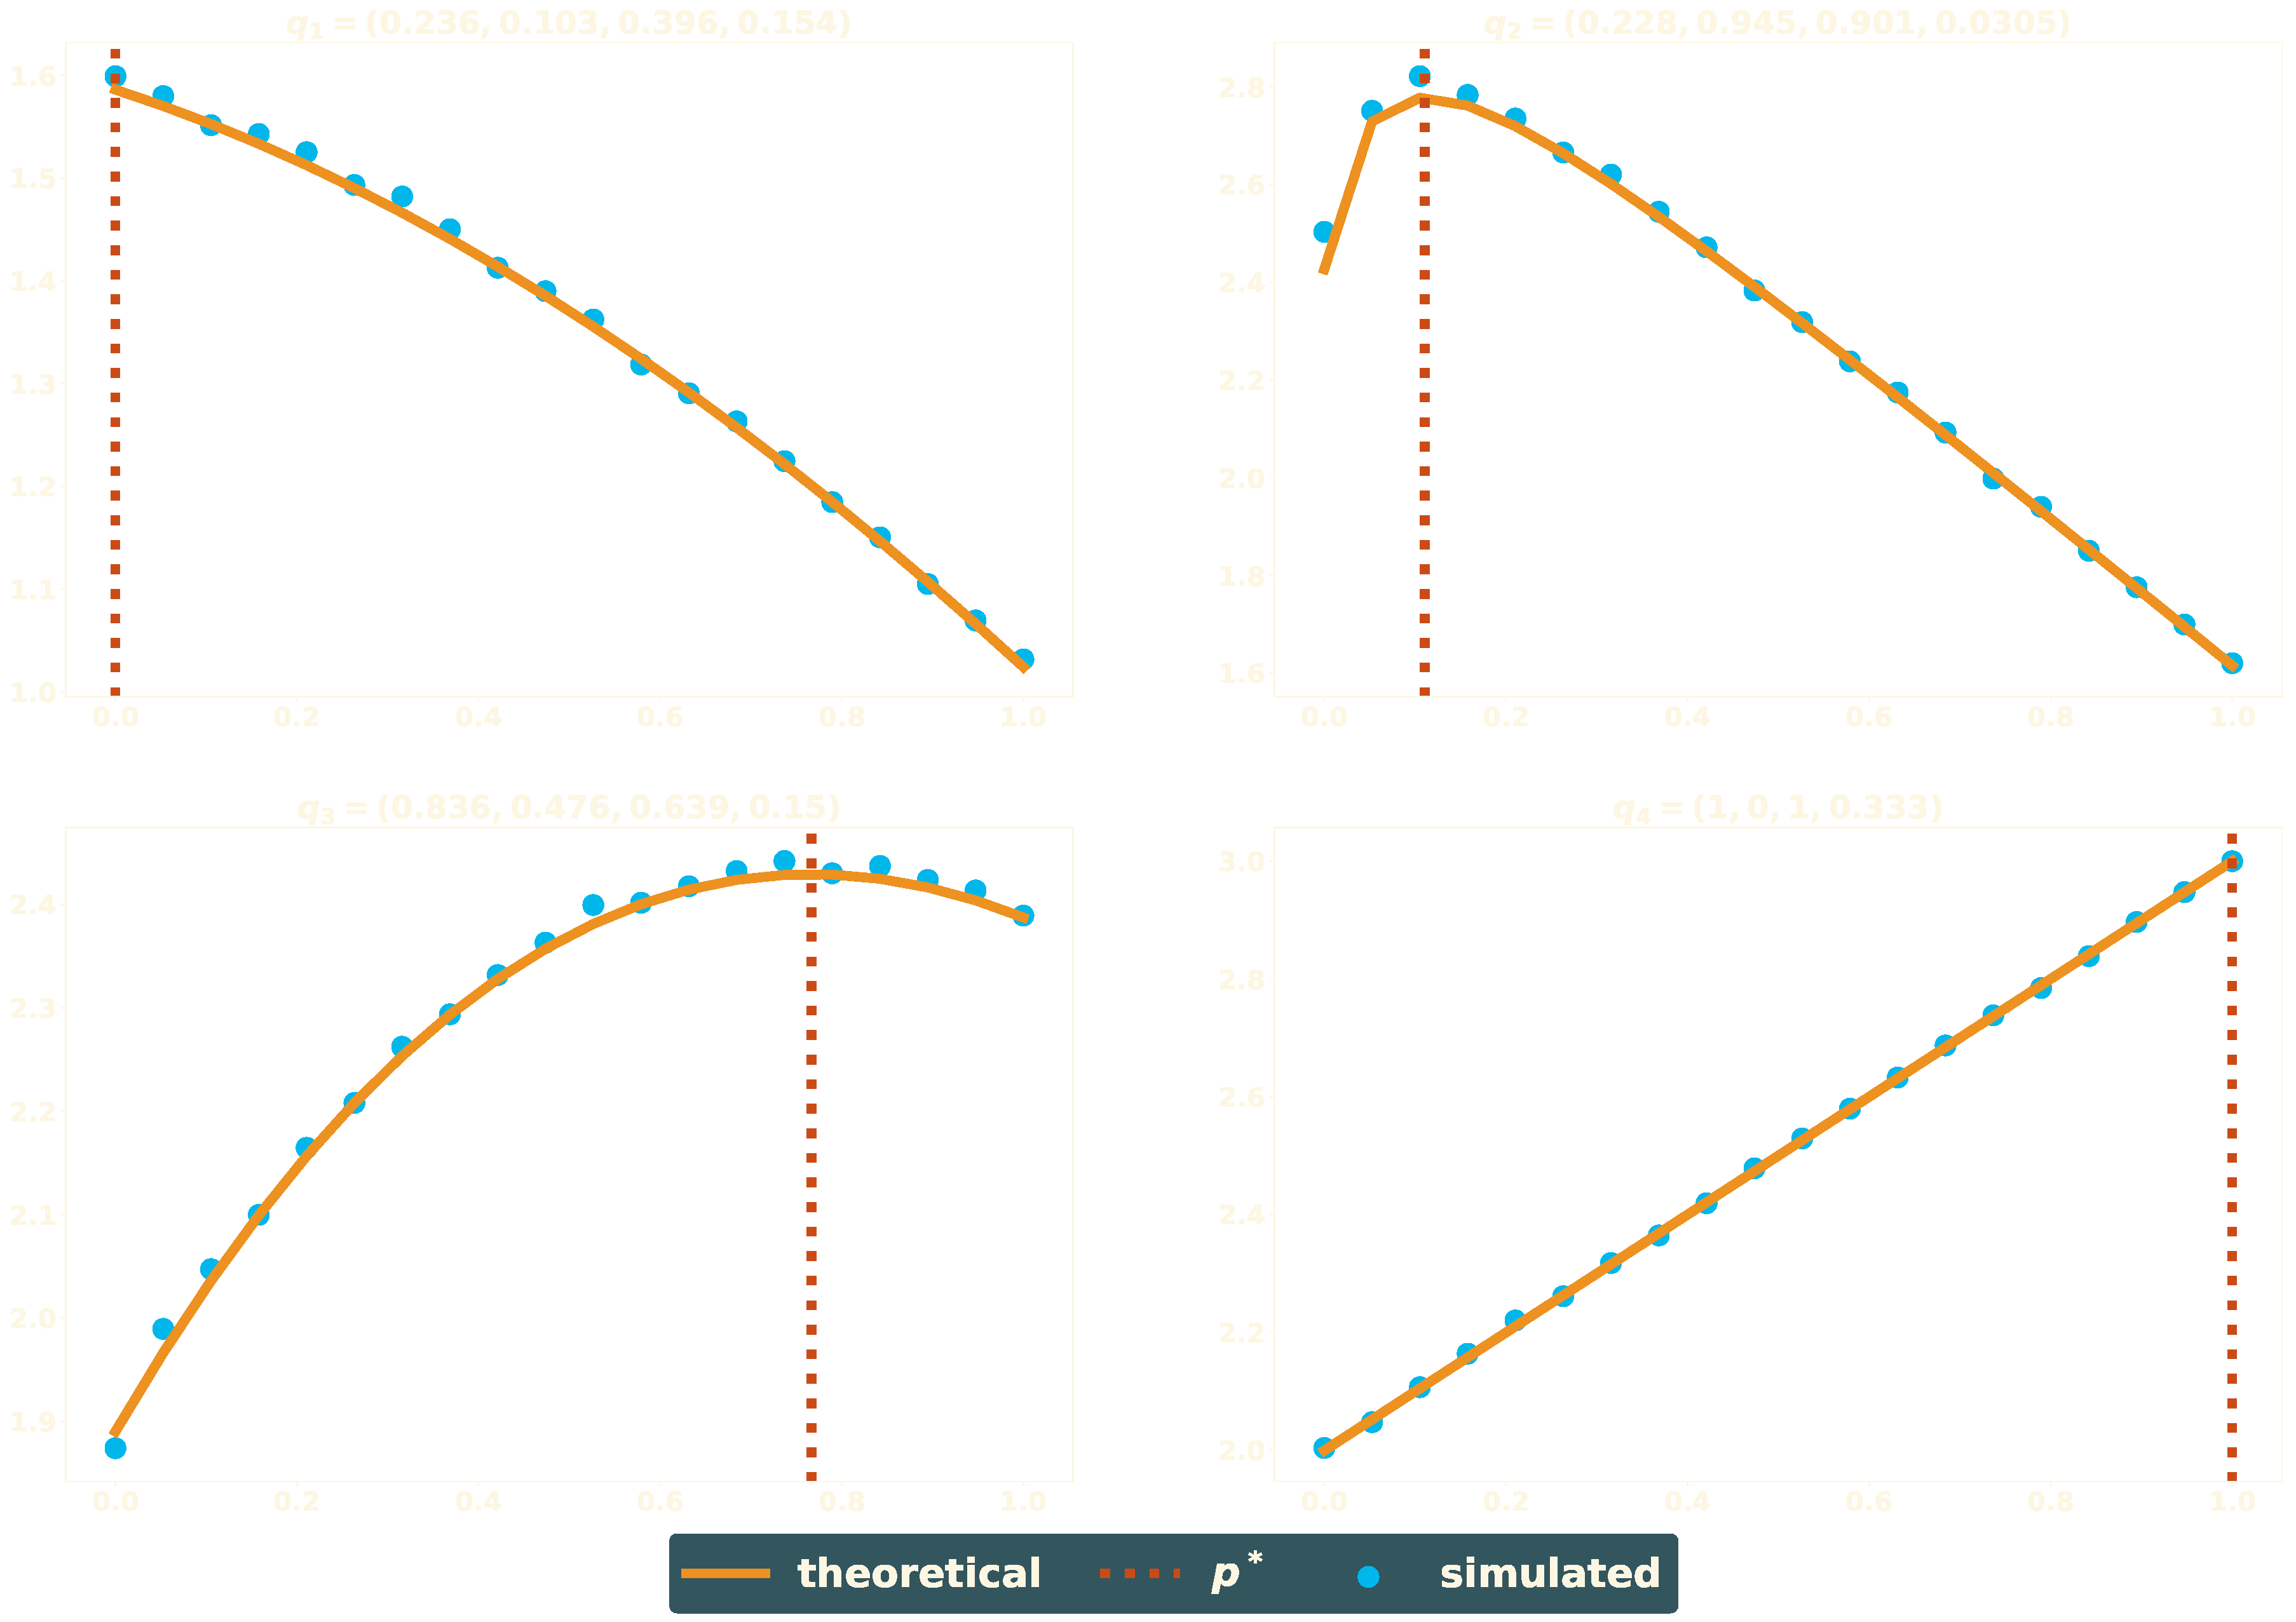
\includegraphics[width=.7\textwidth]{static/matches}
            \end{center}
        \end{column}
        \begin{column}{.5\linewidth}
            \begin{center}
                \vspace{-1cm}
    
                \textcolor{orange}{\textbf{\small{AGAINST MULTIPLE OPPONENTS}}}
                \vspace{2cm}
    
                \includestandalone[width=.7\textwidth]{static/multiple_opponents}
                \vspace{-.5cm}
                
                \textbf{\[u_q(p)\]} \\
                \includestandalone[width=.02\textwidth]{static/arrow_down} \\
                \footnotesize{
\(
\left[\begin{matrix}
    0 \enspace & 0 \enspace & \dots \enspace & 0 \enspace & -a_{0}\\
    1 \enspace & 0 \enspace & \dots \enspace & 0 \enspace & -a_{1} \\
    \vdots \enspace & \vdots \enspace & \ddots \enspace & \vdots  \enspace & \vdots \\
    0 \enspace & 0 \enspace &  \dots  \enspace & 1 \enspace & -a_{2N}
\end{matrix}\right]
\)
} \\
                \includestandalone[width=.02\textwidth]{static/arrow_down} \\
                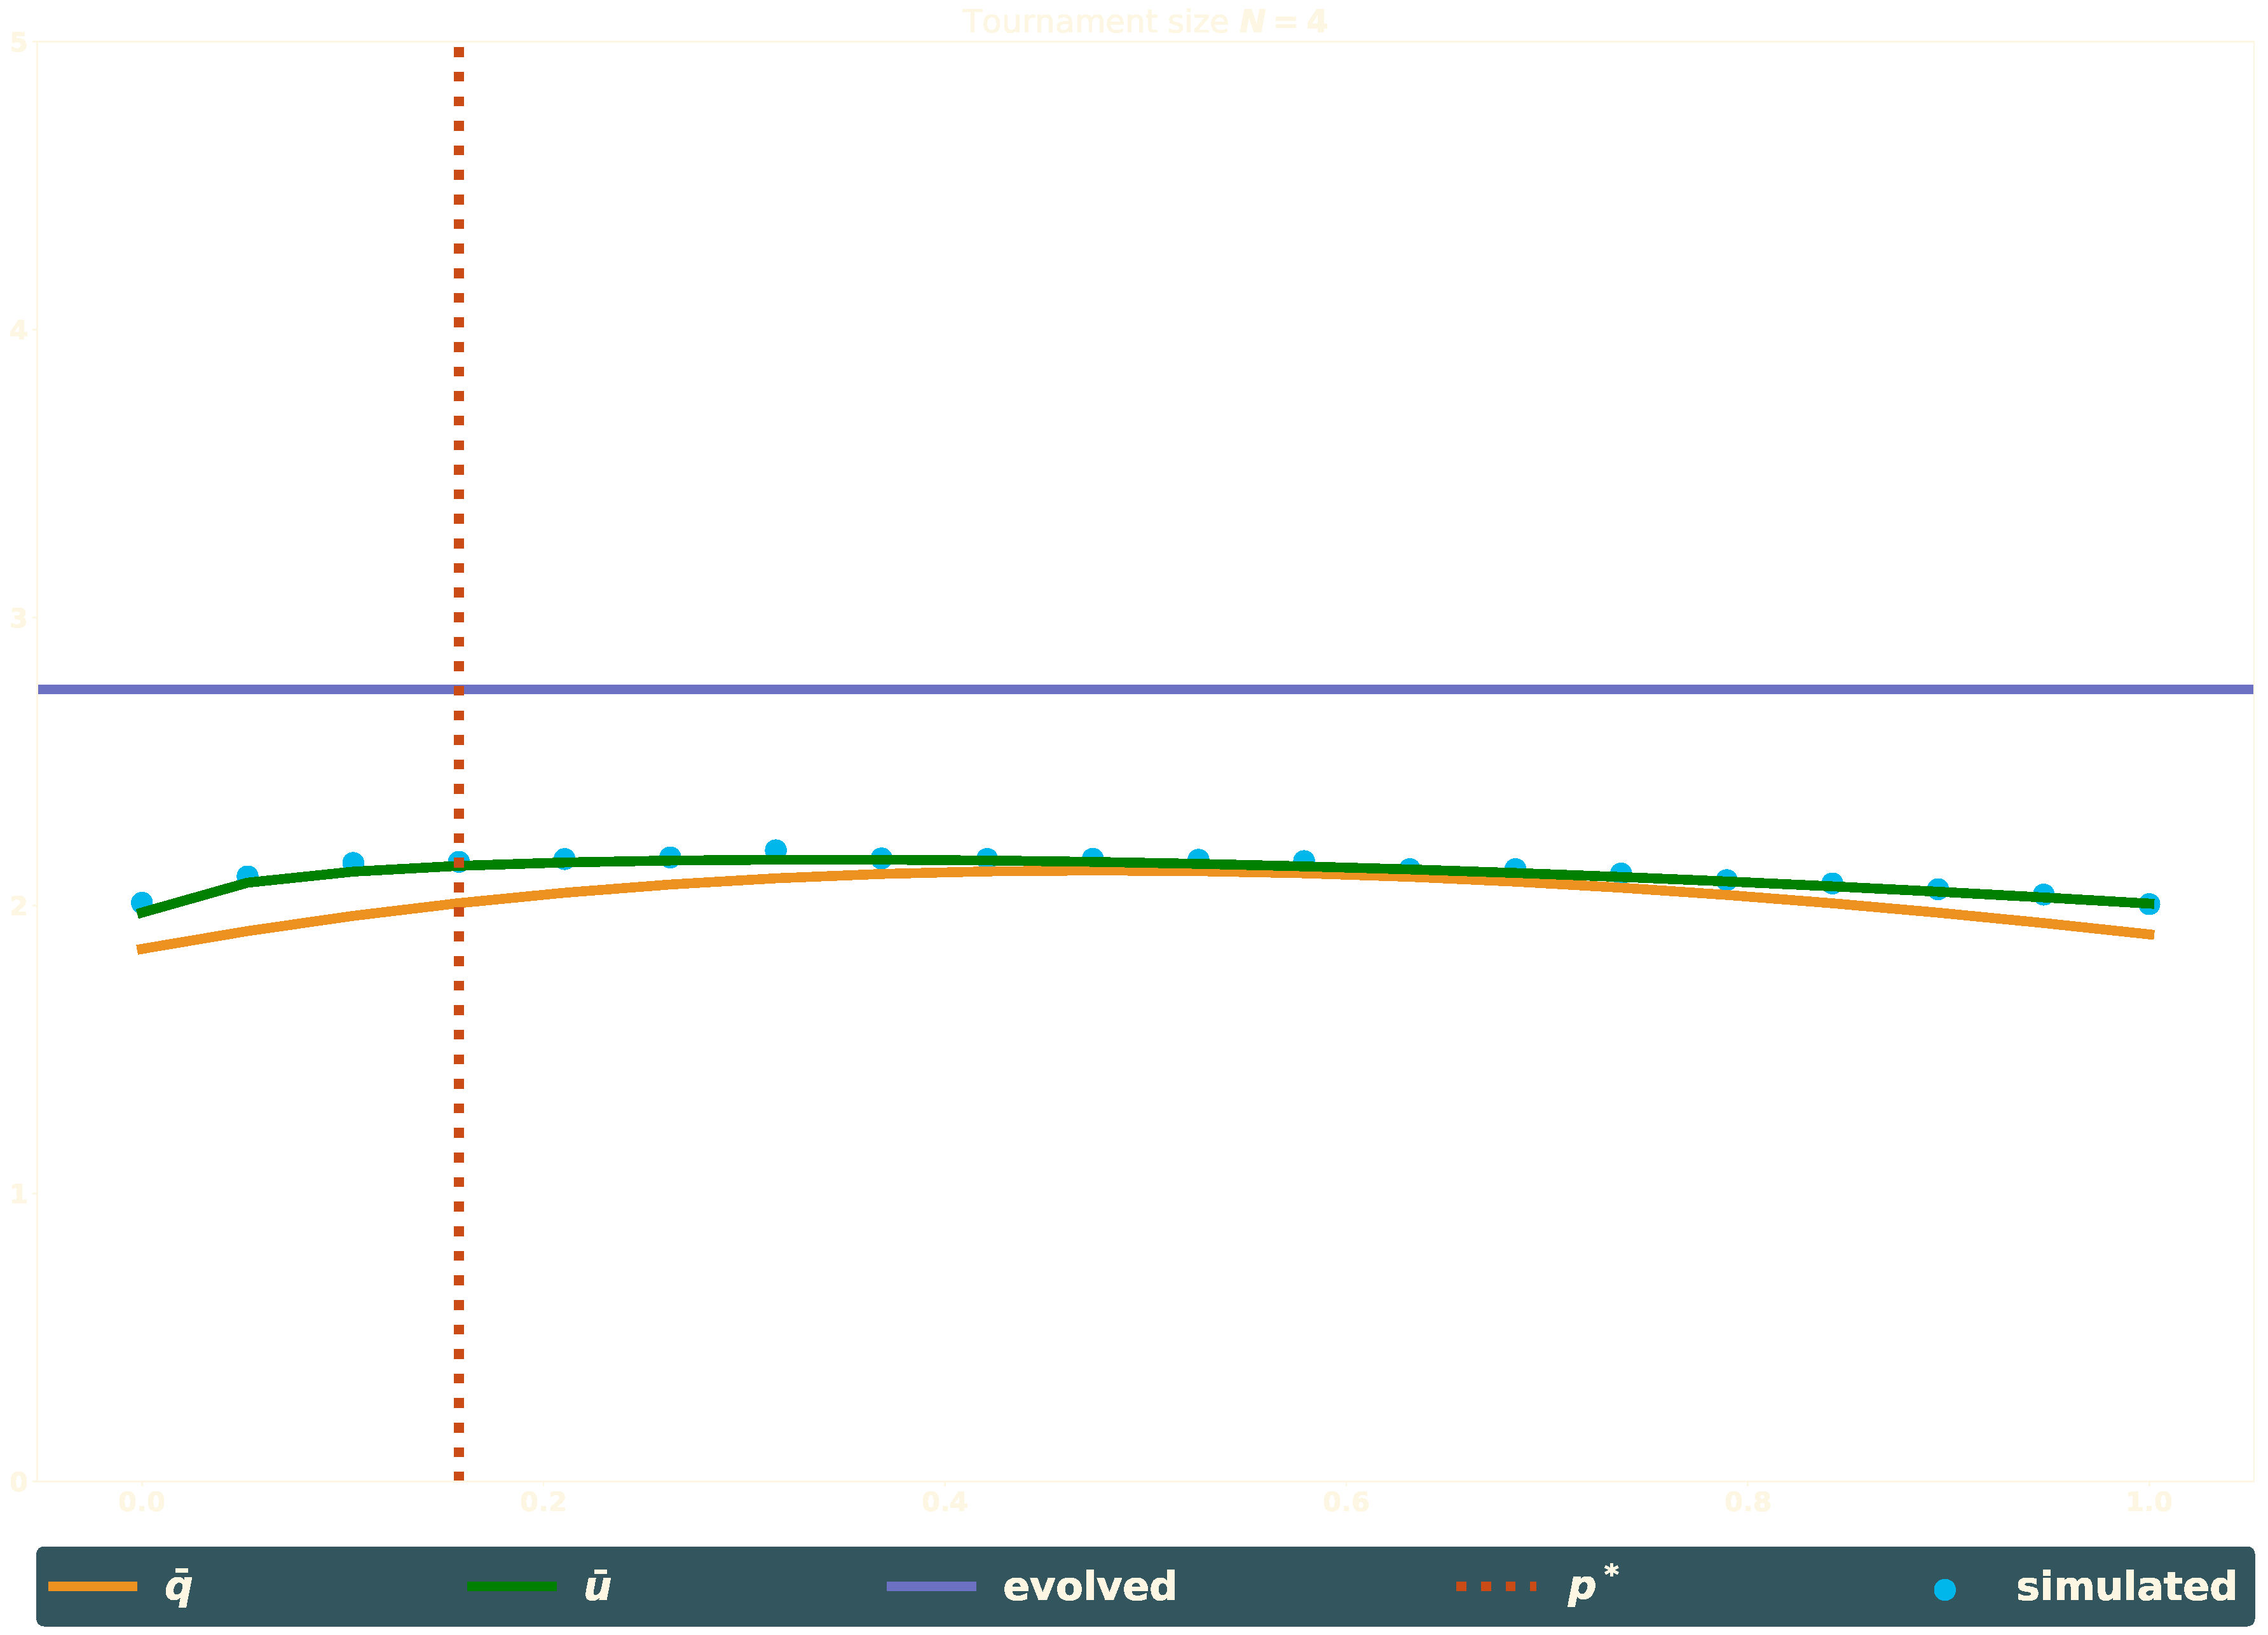
\includegraphics[width=.5\textwidth]{static/tournament}

            \end{center}
        \end{column}
    \end{columns}
    \end{column}
    \begin{column}{.2\linewidth}
        \begin{center}
            \textcolor{orange}{\textbf{\Large{FUTURE WORK}}} \\
            \textcolor{orange}{\textbf{ \(p=(p_1, p_2, p_3, p_4) \rightarrow\) \small{ RESULTANT THEORY}}}
        \end{center}
    \begin{center}
        \includestandalone[width=.6\textwidth]{static/resultant}
    \end{center}
            \vspace{2cm}

            \begin{center}
                \textcolor{orange}{\textbf{\Large{SUMMARY}}}
            \begin{center}
                \begin{enumerate}
                    \item The utility of a given player \(p\) against a given opponent \(q\) 
                    can be written in a compact way.
                    \item Obtaining the optimal random behaviour \(p ^ *\) reduces to a search over a small finite set.
                    \item Optimising against the mean utility can not be captured by optimising against the mean opponent.
                \end{enumerate}
            \end{center}
        \end{center}
    \end{column}
\end{columns}
\vspace{1.5cm}

\hrule height 3pt
%%%%%%%%%%%%%%%%%%%%%%%%%%%%%%%%%%%%%INFO%%%%%%%%%%%%%%%%%%%%%%%%%%%%%%%%%%%%%%%
\begin{columns}
    \begin{column}{.1\linewidth}

        \centering
        \textbf{ \faTwitter \ NikoletaGlyn}
    \end{column}
    \begin{column}{.55\linewidth}

        \centering
        \textbf{ In case you missed me: \url{nikoleta-v3.github.io/blog/2018/01/05/power-of-memory.html}}
    \end{column}
    \begin{column}{.1\linewidth}

        \centering
        \textbf{ \faGithub \ Nikoleta-v3}
    \end{column}
    \begin{column}{.1\linewidth}

        \centering
        \textbf{Cardiff University}
    \end{column}
\end{columns}
\end{document}
